\section{Softwarová část}

\subsection{Typy řízení vytápění}
V rámci řídicího systému existují tyto typy řízení:

\begin{itemize}
  \item Řízení vytápění podle chodbových termostatů.
  \item Řízení vytápění podle nástěnných snímačů prostorových teplot.
  \item Řízení vytápění podle teplotních plánů.
  \item Řízení vytápění podle teplotních plánů s úpravou podle předpovědi počasí.
\end{itemize}

Předpokládá se, že centrální zásobník otopné vody je průběžně ohříván během dne pomocí přebytků energie přes výměníky u krb. Tím se tedy předpokládá, že zásobník je nahřán pro případné potřeby vytápění. Je kladena priorita na získávání ohřáté otopné vody ze zdroje tepla zmíněná dříve. Uživatelé jsou upozorňováni signalizací na displejích jak u krbů, tak i na nástěnných snímačích prostorové teploty, přímo v řídícím systému (možné i notifikace na mobil, e-mail) či LED diodami (rozsvícení všech) u krbů, že je potřeba zatopit v krbech, pokud systém vyhodnotí, že je potřeb vytápět. V případě, že tomu k tomu nedojde využívá se plynový kondenzační kotel, který dohřívá zásobník (ten je možný ovládat automaticky).

V části \textbf{přehled} je pro přehlednost jsou jednotlivé teploty zobrazeny v části „jednotlivé teploty“, jsou zde všechny teploty snímané v zásobníku otopné vody, teploty na kouřovodech v přízemí a patře, v neposlední řadě jez zde i venkovní teplota. V části „porovnání teploty“ jsou zmíněné teploty zobrazeny v jednom grafu.

V části \textbf{nastavení} je možné v \textit{řízení teploty} vybrat jeden typ řízení vytápění (viz výše). Dále v \textit{módy řízení} je výběr módů a to zimní, letní nebo výběr podle venkovní teploty. Výběr módu má vliv na výběr mezních teplot pro spínání plynového kondenzačního kotle. Dané teplotní meze se dají nastavit v~části \textit{spínání plynového kotle} (teplotní meze pro léto a zimu). Tyto nastavené meze se berou pro kontrolu s teplotou v horní části zásobníku otopné vody. Pokud teplota v~horní části zásobníku je menší než teplota definovaná v části „min. zapnutí“ dojde k zapnutí kotle pro nahřátí otopné vody, kotel se vypíná při teplota definované v části „max. vypnutí“. Při porovnávání teplot se též bere v potaz nastavená hystereze v části \textit{ostatní nastavení}. Při výběru módu podle venkovní teploty dochází k automatickému výběru letního nebo zimního módu. Teplotní mez pro výběr letního módu (v rámci módu podle venkovní teploty) je definovaná v části „min. venkovní teplota pro letní mód“. Toto spínání kotle nastává v momentě, kdy po upozornění uživatelů nedojde k zatopení v krbech.

V části nastavení \textit{krby – spínání čerpadel} se definují minimální hranice teploty, kdy dojde k sepnutí oběhových čerpadel pro krbové výměníky, tedy při jaké teplotě se má brát v potaz, zda někdo v krbu zatopit a mají se spustit čerpadla pro nahřívání zásobníku otopné vody. Toto nastavení je poměrně důležité a kontrola těchto teplot je zcela nezávislá na dalších nastaveních (automatizaci) v systému, je potřeba vždy při zatopení spustit čerpadla, jinak dojde k přehřátí vody ve výměníku krbu. V případě přehřátí se aktivuje ochrana přímo u krbů a dojde k ke zvukové signalizaci přehřátí, pokud teplota neklesne za určitou dobu, dojde k aktivování ochranných ventilů a vypuštění přehřáté vody.


V části \textit{LED indikace – mezní parametry zásobníku otopné vody} se definují mezní teploty pro horní, střední a spodní část zásobníku otopné vody. Tato signalizace se zejména týká pro krby, aby uživatel věděl, zda může topit a jak je moc zásobník nahřátý. U modré LED se definuje mezní minimální teplota, kterou by zásobníku ve horní části měl mít (povolení pro topení). U oranžové LED se definuje mezní maximální teplota, kdy ve střední části zásobníku dochází k dostatečnému nahřátí otopné vody (oznámení, že za chvilku by se mělo přestat topit). U červené LED se definuje mezní maximální teplota, kdy ve spodní části zásobníku je plně ohřátá(okamžitě přestat topit.). Aktivace červené LED předchází v dostatečném předstihu před aktivováním ochrany u~krbů pro přehřátí otopné vody, popsáno v předchozím odstavci.
\subsubsection{Řízení vytápění podle chodbových termostatů}
V přízemí a v patře je na chodbě umístěn jeden lokání termostat popsaný v části \ref{sec:digitalni-chodbove-termostaty}. Tento termostat na základě lokálního nastavení (není součástí řídicího systému) spínání/rozpínání výstupní relé při požadavku na vytápění. Tento požadavek se následně vyhodnotí v centrálním systému a dojde k sepnutí nebo rozepnutí daného chodbového oběhového čerpadlo pro podlahové vytápění a otevření všech okruhů podlahové vytápění. Dochází tedy k řízení vytápění všech místností na patře podle jednoho centrálního termostatu. 

\subsection{Záložka zařízení}
V části „koncová zařízení“ se zobrazují jednotlivá ovládána (zapnuto/vypnuto) zařízení otopné soustavy, tedy plynový kondenzační kotel, čerpadla pro krby s výměníkem, čerpadla pro podlahové vytápění a zapnutí signalizačních LED u krbů. Je možné samotnou automatizaci respektive ovládání zmíněných zařízení řídit podle vlastního uvážení, proto slouží přepínač „manuální ovládání zařízení“, zde si pak uživatel může libovolně jednotlivá zařízení ovládat bez ohledu na nastavenou automatizaci.

V části „termostaty chodby – požadavek topení“, zde se zobrazuje zda dochází k vytápění v přízemí či patře na základě nastavení lokálních termostatů na chodbách.

V části „ovládání čerpadel – vodní kámen“ slouží ke spínání čerpadel pro ochranu před zatuhnutím lopatek. Vzhledem k místní dosti tvrdé vodě, došlo při netopení v přízemí, tedy při nevyužívání daných čerpadel k zatuhnutí lopatek v důsledku nánosu vodního kamene. Pro se zde nachází nastavení, kde si uživatel může pro konkrétní den, hodinu a definovanou délku nastavit spínání čerpadel pro odstranění nánosu na lopatách. Ideální volbou je otopnou vodu zbavit minerálů nebo vyměnit za destilovanou vodu, nicméně k některým méně kvalitnějším provedením spojům trubek otopné soustavy, by docházelo k průsaku otopné vody. Proto je otopná vody z řádu s vyšším podílem minerálů jedním z řešení, jak docílit zaslepení průsaku především vápníkem bez nutnosti, alespoň prozatím, spoje opravovat.

Výše popsané části jsou zobrazená na obrázku \ref{fig:ha-zarizeni}.




\begin{figure}[H]
    \centering
    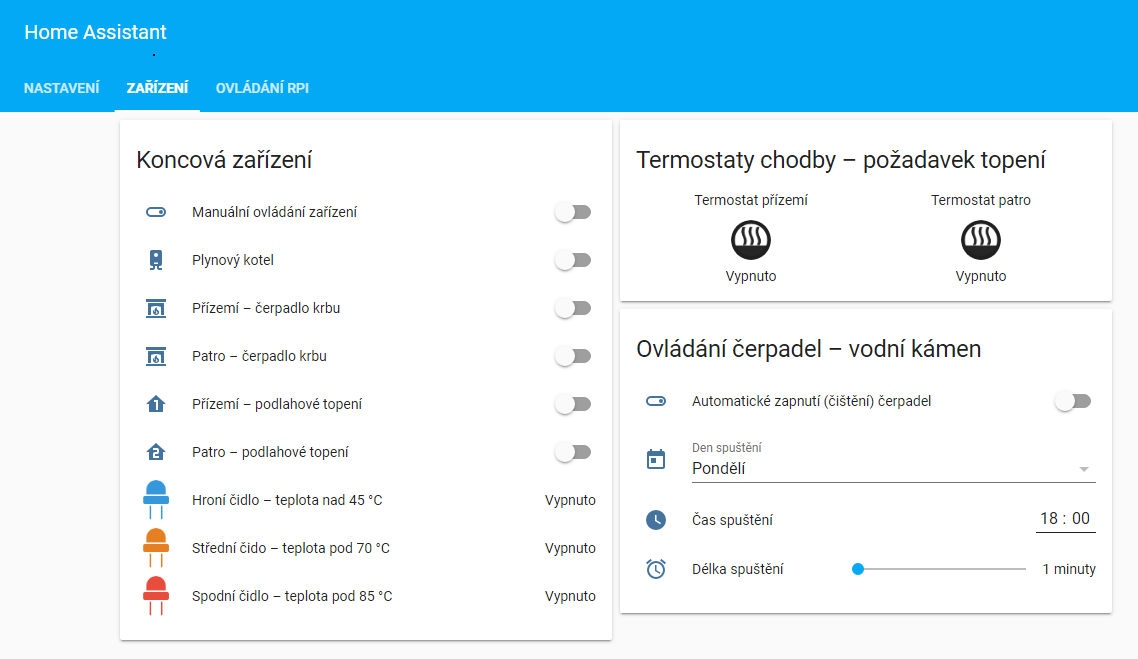
\includegraphics[width=0.90\textwidth]{images/software-ha/ha-zarizeni.png}
    \caption{Záložka zařízení v HA.}
    \label{fig:ha-zarizeni}
\end{figure}

\subsection{Vývoj pro zónovou regulaci}

Na obrázku \ref{fig:teplotni-plan} je zobrazen možný nastavitelný teplotní plán pro celý den. Lze tak nastavit všechny dny v týdnu. Pro každý zvolený teplotní úsek je možné si zvolit požadovanou teplotu.

\begin{figure}[H]
    \centering
    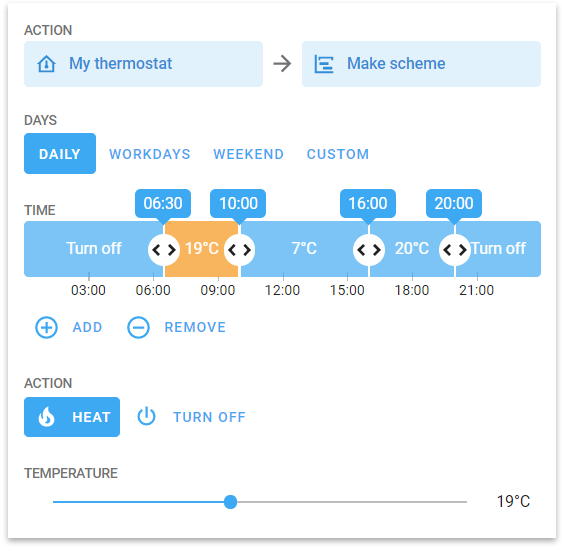
\includegraphics[width=0.90\textwidth]{images/software-ha/teplotni-plan.png}
    \caption{Nastavitelný teplotní plán pro danou hodinu v celém dni.}
    \label{fig:teplotni-plan}
\end{figure}

Na obrázku \ref{fig:termostat-v-mistnosti} je nastavení aktuální teploty pro požadovanou místnost. Každá místnost má svoje vlastní nastavení. Zobrazuje se zde aktuálně naměřená teplota v dané místnosti a požadovaná teplota. Pokud dojde k~přenastavení požadované teploty, dojde k přenesení této teploty do nástěnného snímače prostorové teploty, přenos funguje i opačně.

\begin{figure}[H]
    \centering
    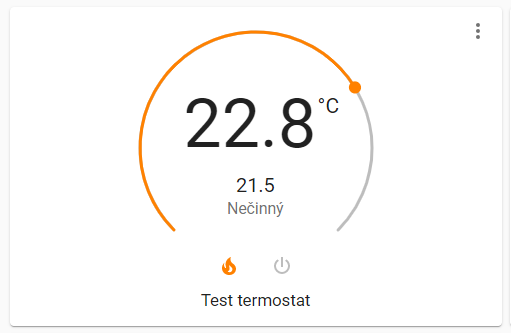
\includegraphics[width=0.90\textwidth]{images/software-ha/termostat-v-mistnosti.png}
    \caption{Zobrazení aktuální teploty z dané místnosti, možnost nastavit požadovanou teplotu.}
    \label{fig:termostat-v-mistnosti}
\end{figure}


